\documentclass{article}
    % General document formatting
    \usepackage[margin=0.7in]{geometry}
    \usepackage[parfill]{parskip}
    \usepackage[utf8]{inputenc}
    
    % Related to math
    \usepackage{amsmath,amssymb,amsfonts,amsthm}
\usepackage{graphicx}
%\usepackage{subfig}
%\usepackage{subfigure}
\usepackage{caption}
\usepackage{subcaption}
\usepackage{listings}
\usepackage{braket}
\usepackage{gensymb}

\usepackage{titling}
%\usepackage{lipsum}

\usepackage{titlesec}

\titleformat*{\section}{\Large\bfseries}
\titleformat*{\subsection}{\large\bfseries}
%\titleformat*{\subsubsection}{\large\bfseries}
%\titleformat*{\paragraph}{\large\bfseries}
%\titleformat*{\subparagraph}{\large\bfseries}
\titlespacing\section{0pt}{12pt plus 4pt minus 2pt}{0pt plus 2pt minus 2pt}
\titlespacing\subsection{0pt}{12pt plus 4pt minus 2pt}{0pt plus 2pt minus 2pt}
\titlespacing\subsubsection{0pt}{12pt plus 4pt minus 2pt}{0pt plus 2pt minus 2pt}

\pretitle{\begin{center}\large\bfseries}
\posttitle{\par\end{center}\vskip 0.01em}
\preauthor{\begin{center}\Large\ttfamily}
\postauthor{\end{center}}
\predate{\par\normalsize\centering}
\postdate{\par}

\title{Population Genetic Analyses of Genomic Data 1}
%\date{\today}


\begin{document}

%\maketitle

\begin{center}
\textbf{\LARGE{\centering{Computational Neuroscience 2}}}\\

\textit{USN: 303039534}\\
\end{center}

%\normalsize{   }

\section{Unsupervised learning}

For a general many-input-one-output network we can define an input vector \textbf{u} as the activity of the neurons in the input layer and a weight vector \textbf{w} as the strength of connections between the input neurons and the output neuron. The total input to the output neuron is thus
$ v = \bf{w} \cdot \bf{u} $.

Based on Hebb's conjecture from 1949, we can write a simple learning rule where the strength of a synapse increases with correlated pre- and post-synaptic coactivity:
\begin{equation}
\tau_w \dfrac{d\bf{w}}{dt} = v \bf{u}
\end{equation}
If we assume that synaptic weight changes occur over a much slower timescale than the inputs, we can use 'batch learning' and average over all input data in every learning step:
$
\tau_w \dfrac{d\bf{w}}{dt} = \braket{v \bf{u}}
$.
Since $v = \bf{w} \cdot \bf{u} $ and defining the correlation matrix ${\bf Q} = \braket{{\bf u u} }$, this allows us to learn weights using simple matrix multiplication
\begin{equation}\label{eq:batchlearn}
\tau_w \dfrac{d\bf{w}}{dt} = \bf Q \cdot w
\end{equation}
Note that this definition of 'correlation' is slightly odd, as for example the self correlation is given by $Q_{ii} = \braket{u_i^2}$ rather than self correlations always being 1.
We then continue to iterate over equation \ref{eq:batchlearn} until the weights have converged. If the activities of our neurons correspond to firing rates, all $u_i$ must be positive. The correlation matrix is therefore a non-negative matrix and we cannot learn negative correlations. Instead, it is therefore common to use a covariance-based learning rule where we let $\bf u' = u-\braket{u}$. Now defining the covariance matrix ${\bf C} = \braket{( {\bf u} - \braket{\bf u})  ( {\bf u} - \braket{\bf u})}$ we can rewrite our learning rule as
\begin{equation}\label{eq:cov}
\tau_w \dfrac{d\bf{w}}{dt} = \bf C \cdot w
\end{equation}
We note that since these batch learning rules are linear in \textbf{w}, we can treat them analytically.
At any given time, we can decompose the weight vector in terms of the eigenvectors $e_\mu$ of \textbf{C}:
\begin{equation}
{\bf w}(t) = \sum_\mu{ c_\mu(t) {\bf e}_\mu }
\end{equation}
Solving the linear differential equation \ref{eq:cov} we get
$
c_\mu = \exp{( \dfrac{\lambda_\mu t}{\tau_w})}({\bf w}(0) \cdot {\bf e_\mu})
$
and putting these results together gives
\begin{equation}\label{eq:anal}
{\bf w}(t) = \sum_\mu{ \exp{( \dfrac{\lambda_\mu t}{\tau_w})}({\bf w}(0) \cdot {\bf e_\mu})  {\bf e}_\mu}
\end{equation}
If the covariance matrix is non-degenerate, we expect the eigenvector corresponding to the highest eigenvalue to dominate this sum at long times due to the coefficient being exponential in the eigenvalue. This in turn suggests that the weight vector will converge towards this first principal component unless it is orthogonal to the initial weight matrix.
However, this basic Hebbian learning will lead to unphysiological unbounded weight increases and is therefore usually augmented with some sort of normalization which can alter the simple behavior expected from equation \ref{eq:anal} as will be evident from the next two sections.

We note that since the timescale is arbitrary for the above equations, we can set $\tau_w = 1$ for the remainder of this section without loss of generality. We require dt to be smaller than $\tau_w$ for accurate Euler integration and therefore let dt=0.01. This is equivalent to using a discrete learning rule with $\epsilon = \dfrac{dt}{\tau_w}=0.01$.

\subsection{Multiplicative normalization}

One commonly used form of normalization is multiplicative normalization where we subtract a term from the simple Hebbian learning rule proportional to the current weights at each iteration. We implement this using Oja's learning rule:
\begin{equation}\label{eq:ojacont}
\tau_w \dfrac{d\bf{w}}{dt} = v {\bf{u}} - \alpha v^2 {\bf{w}}
\end{equation}
To see how this leads to normalization, we take the dot product of equation \ref{eq:ojacont} with \textbf{w}
\begin{equation}
\tau_w \dfrac{d|{\bf{w}}|^2}{dt} = v {\bf{w} \cdot \bf{u}} - \alpha v^2 {\bf{w} \cdot \bf{w}} = v^2(1-\alpha |{\bf{w}}|^2)
\end{equation}
Hence $\dfrac{d|{\bf{w}}|^2}{dt} \rightarrow 0$ as $\alpha |{\bf{w}}|^2 \rightarrow 1$ and Oja normalization constrains the modulus of the weight vector. At long times, we thus converge towards a weight vector of magnitude $|{\bf{w}}| \rightarrow \dfrac{1}{\sqrt{\alpha}}$. In the following, we let $\alpha=1$ such that the weight vector converged to is normalized.

As above, we average over the training inputs and get a batch learning rule
\begin{equation}\label{eq:oja}
\tau_w \dfrac{d\bf{w}}{dt} = {\bf Q \cdot w} - \alpha ({\bf w \cdot Q \cdot w}) {\bf w}
\end{equation}
We then update weights according to equation \ref{eq:oja} until the norm of the change in weights between iterations is $\epsilon < 10^{-6}$. Setting $\alpha=1$ we note that when \textbf{w} becomes an eigenvector of \textbf{Q} with eigenvalue $\lambda$, we can write ${\bf Q \cdot w} = \lambda \bf w$ and $({\bf w \cdot Q \cdot w}) = \lambda$, giving  $\tau_w \dfrac{d\bf{w}}{dt} =0$. For Oja's rule, we thus expect the weight vector to converge to an eigenvector of \textbf{Q}, and we expect this to be the largest eigenvector on the basis of equation \ref{eq:anal}.

We see an example of this in figure \ref{fig:sim1mul} where we train the network on a two-dimensional Gaussian dataset with each point corresponding to a two-dimensional input datapoint \textbf{u}. The red line indicates the direction of the final weight vector, shifted vertically to run through the mean of the dataset, and we see that it does indeed align with the first principal component (the axis of maximum variability).

However, if we shift the mean of the gaussian input dataset to (3,3), the correlation matrix \textbf{Q} becomes a positive matrix and the largest eigenvalue now corresponds to the eigenvector (1,1) although there is still a negative covariance between the x and y component of the data (figure \ref{fig:sim2mul}). In this case, the converged weight vector thus ends up being perpendicular to the first principal component of the data.

However, we can salvage this behavior by using the covariance-based learning rule from equation \ref{eq:cov} on the same dataset (figure \ref{fig:sim3mul}). This allows us to once again capture the negative covariance between the components $u_1$ \& $u_2$ as the converged weight vector aligns with the first principal component of the data.

\begin{figure}[h]
	\centering
	\begin{subfigure}[t]{0.30\linewidth}
		\centering
		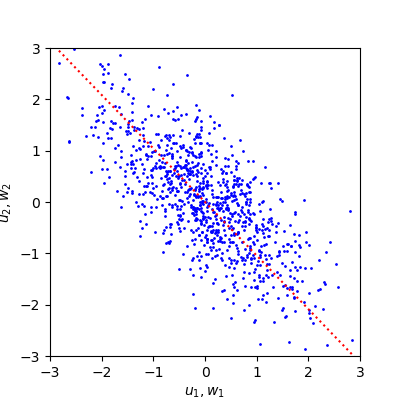
\includegraphics[width = 1.0\linewidth, trim={0 0 0 0}, clip=true]{figures/2d_sim1.png}
		\subcaption{Mean (0,0) with correlation-based training. Final weight vector: [0.692, -0.722], principal components: [-0.692, 0.722] \& [-0.722, -0.692]}
		\label{fig:sim1mul}	
	\end{subfigure}%
	\hspace{0.03\linewidth}
	\begin{subfigure}[t]{0.30\linewidth}
		\centering
		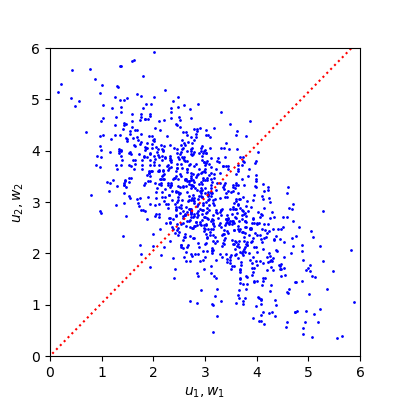
\includegraphics[width = 1.0\linewidth, trim={0 0 0 0}, clip=true]{figures/2d_sim2.png}
		\subcaption{Mean (3,3) with correlation-based training. Final weight vector: [-0.697, -0.717], principal components: [-0.696, 0.718] \& [-0.718, -0.696]}
		\label{fig:sim2mul}	
	\end{subfigure}%
	\hspace{0.03\linewidth}
	\begin{subfigure}[t]{0.30\linewidth}
		\centering
		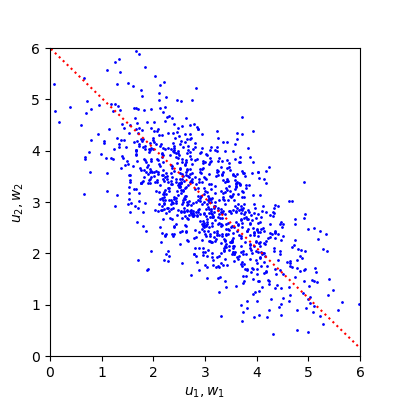
\includegraphics[width = 1.0\linewidth, trim={0 0 0 0}, clip=true]{figures/2d_sim3.png}
		\subcaption{Mean (3,3) with covariance-based training. Final weight vector: [0.716, -0.698], principal components: [-0.716, 0.698] \& [-0.698, -0.716]}
		\label{fig:sim3mul}	
	\end{subfigure}%
\caption{Learning weight vectors from 500 input data points with Oja's rule. In each case, we start from [w1, w2] = [0.001, 0.001] and iterate through equation \ref{eq:oja} until convergence using either a correlation or covariance-based learning rule. Red dotted lines indicate the direction of the final weight vector. All datasets were generated with a slope of 1, a standard deviation of 1 and $1-\rho^2$ in the $u1$ and $u2$ directions, and a correlation of $\rho = -0.7$.}
\label{fig:multiplicative}
\end{figure}

If instead we were to have a positive covariance between the $u1$ and $u2$ components of our input vectors, the final weight vector aligns with the principal component irrespective of whether the mean of our distribution is zero, positive or negative provided that the mean of both the u1 and u2 components have the same sign. In this case we instead fail to recover the first principal component in the case where the mean of the $u1$ is positive while the mean of u2 is negative or vice versa. In that case we get a final vector of [0.692, -0.722] despite a first principal component of [0.689, 0.725] in an example simulation. This is again salvaged by using a covariance-based learning rule.

We can also investigate the magnitude of our weight vectors over time since we expect these to converge smoothly to 1 as discussed above, and we see that this is indeed the case (figure \ref{fig:multiplicativevec}). Interestingly, it appears that convergence to the [1,1] vector in our second simulation is much faster than converging to a [-1, -1] vector in simulations 1 \& 2.

\begin{figure}[h]
	\centering
	\begin{subfigure}[t]{0.30\linewidth}
		\centering
		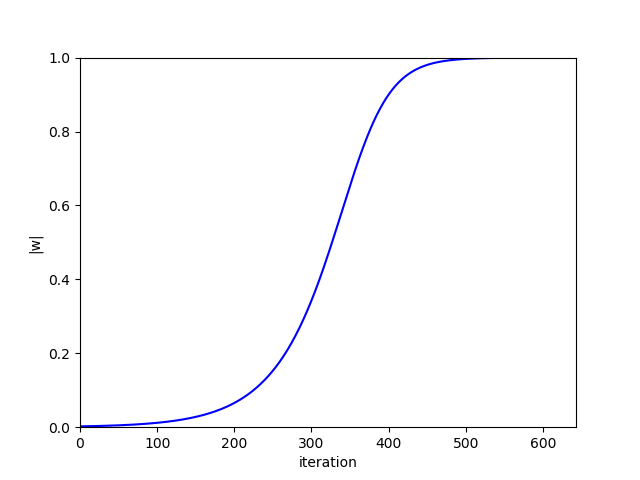
\includegraphics[width = 1.0\linewidth, trim={0 0 0 0}, clip=true]{figures/2d_sim1_vec.png}
		\subcaption{}
		\label{fig:sim1vec}	
	\end{subfigure}%
	\hspace{0.03\linewidth}
	\begin{subfigure}[t]{0.30\linewidth}
		\centering
		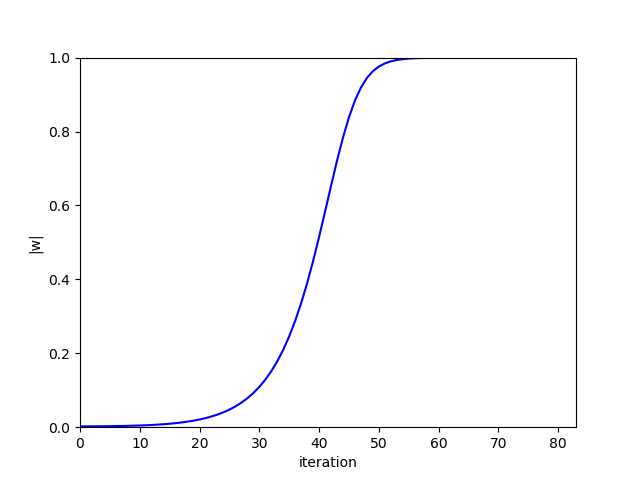
\includegraphics[width = 1.0\linewidth, trim={0 0 0 0}, clip=true]{figures/2d_sim2_vec.png}
		\subcaption{}
		\label{fig:sim2vec}	
	\end{subfigure}%
	\hspace{0.03\linewidth}
	\begin{subfigure}[t]{0.30\linewidth}
		\centering
		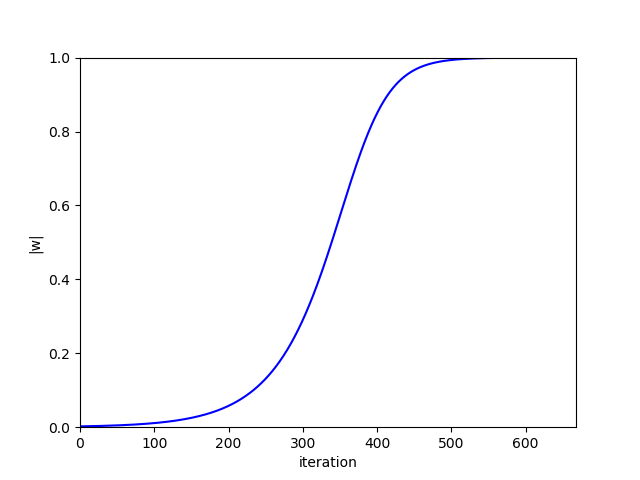
\includegraphics[width = 1.0\linewidth, trim={0 0 0 0}, clip=true]{figures/2d_sim3_vec.png}
		\subcaption{}
		\label{fig:sim3vec}	
	\end{subfigure}%
\caption{Weight vector magnitude as a function of iteration number for the three simulations in figure \ref{fig:multiplicative}}
\label{fig:multiplicativevec}
\end{figure}

\subsection{Subtractive normalization}

A different form of normalization that is commonly used to prevent excessive growth of weights is subtractive normalization as specified in equation \ref{eq:subcont}.

\begin{equation}\label{eq:subcont}
\tau_w \dfrac{d\bf{w}}{dt} = v {\bf{u}} - \dfrac{v(\bf{n}\cdot {\bf{u}}) {\bf{n}}}{N_u}
\end{equation}
This constrains the sum of the weights to be constant as can be proven by taking the dot product with \textbf{n} where \textbf{n} is a vector of ones:
\begin{equation}
\tau_w \dfrac{d\bf{n} \cdot \bf{w}}{dt} = \tau_w \dfrac{d\sum_i{w_i}}{dt} = v{\bf{n}} \cdot {\bf{u}}(1 - \dfrac{\bf{n}\cdot {\bf{n}}}{N_u}) = 0
\end{equation}

The total sum of the weights in the system is thus constant, but these weights must still be thresholded to avoid unbounded growth of complementary weights towards $\pm \infty$. This is commonly achieved by constraining all weights to be $\geq 0$ in which case there is an upper saturation limit of $w_{max} = \sum_i{w_i(0)}$.

We once again average our learning rule from equation \ref{eq:subcont} over the training data and get

\begin{equation}\label{eq:subavg}
\tau_w \dfrac{d\bf{w}}{dt} = {\bf Q \cdot w} - \dfrac{({\bf w \cdot Q \cdot n}) {\bf n} }{N_u}
\end{equation}

This is a highly competitive learning rule, and we therefore observe convergence to weights of [1,0] or [0,1] depending on initial conditions in the vast majority of cases, including the three datasets in figure \ref{fig:multiplicative} and equivalent datasets with positive $\rho$ (data not shown).
Even using identical initial weights, we will still converge to [0,1] or [1,0] rather than obeying the symmetry of the initial weights, since the data is noisy which leads to our covariance and correlation matrices having non-identical diagonal elements, leading to symmetry breaking. 

However, there exist a few special cases where we observe different behavior or where the weights still align with the principal components. One such case is where the data has a principal component that is either [0,1] or [1,0]. As an example, we alter our 2d Gaussian function to generate data with a specified slope between the x and y components and construct a 2d Gaussian with slope 0 and rho=0.995. The correlation matrix now has principal components of [1.0, 0.0] \& [0.0, 1.0] and our weights evolve from [0.5, 0.5] to [1.0, 0] over the course of the simulation. In this case we thus do recover our first principal component.

Another special case is when the system is initialized at a fixed point. The fixed point of this system is given by
\begin{equation}
w_2 = \dfrac{Q_{11}-Q_{12}}{Q_{22}-Q_{12}}w_1
\end{equation}
This is an unstable fixed point, but if we initialize the weights at exactly these values, they will remain there indefinitely due to both derivatives being 0. If this vector matches the first principal component of the data, the long term behavior of the weight vector will also be to match this principal component. This is achieved when $u_1$ and $u_2$ are positively correlated with a slope of 1 and equal autocorrelations such that $w_1$ = $w_2$ is the fixed point and first PC.

In these two cases, we thus observe produce a weight vector aligned with the principal component axis of the dataset, and otherwise we do not.
To illustrate this, we run 500 simulations with random initial vectors constrained by $w_1 + w_2 = 1$ and $w_1, w_2 \in [0,1]$, and with the data having $\rho = 0.7$ and a slope of either 1 or 0.2. We then compare the converged weight vector to the first principal component of the input data by calculating the angle $\theta$ between the two vectors. We plot histograms of these angles in figure \ref{fig:thetas}.

\begin{figure}[h]
	\centering
	\begin{subfigure}[t]{0.30\linewidth}
		\centering
		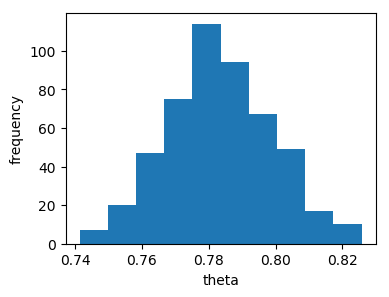
\includegraphics[width = 1.0\linewidth, trim={0 0 0 0}, clip=true]{figures/rho7_slope1_hist.png}
		\subcaption{}
		\label{}	
	\end{subfigure}%
	\hspace{0.1\linewidth}
	\begin{subfigure}[t]{0.30\linewidth}
		\centering
		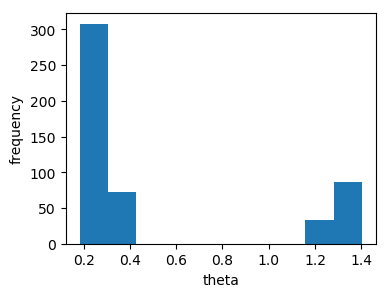
\includegraphics[width = 1.0\linewidth, trim={0 0 0 0}, clip=true]{figures/rho7_slope02_hist.png}
		\subcaption{}
		\label{}	
	\end{subfigure}%
\caption{Histograms of angles between the first PC vector and  the weight vector converged to from a random initial vector when the data has a slope of $1$ (a) or $0.2$ (b).}
\label{fig:thetas}
\end{figure}

We see that there is very little variability in the long-term behavior of the system. In the case of a slope of 1 when the axis of the principal component is on average exactly between the [0,1] and [1,0] vectors, we arrive at a narrow distribution of angles near $\theta = \pi / 4$. When the slope is 0.2, we get two narrow distributions near $\theta = 0.20$ corresponding to a final weight vector of [1,0] and near $\theta = 1.37$ corresponding to a final weight vector of [0,1].

\section{Ocular dominance columns}

In the following, we consider a many-input-many-ouput recurrent circuit with activity vector \textbf{v}, input vector $\bf u$, feedforward weight matrix $\bf W$ and thus total input vector $\tilde {\bf u} = {\bf W \cdot u}$. We additionally let the system have a fixed recurrent weight matrix $\bf M$. The dynamics of this system follow differential equation \ref{eq:occont}
\begin{equation}\label{eq:occont}
\tau_r \dfrac{d \bf v}{dt} = -{\bf v} + {\bf W \cdot u} + {\bf M\cdot v}
\end{equation}
Provided that the eigenvalues of \textbf{M} have real parts $<1$, a stability analysis shows that this system will have a stable fixed point with steady state activity given by 
\begin{equation}
{\bf v} = {\bf W \cdot u} + {\bf M \cdot v}
\end{equation}
Defining ${\bf K} = ({\bf I} - {\bf M})^{-1}$, this has the solution
$
{\bf v} = {\bf K \cdot W \cdot u}
$

If we now fix the recurrent weights and let the feedforward weights change according to a Hebbian learning rule, the time evolution of the weights is determined by equation \ref{eq:ocheb} with $\bf Q$ defined as in section 1.
\begin{equation}\label{eq:ocheb}
\tau_w \dfrac{d{\bf W}}{dt} = \braket{\bf vu} = {\bf K \cdot W \cdot Q}
\end{equation}
We will use a discretized form of this equation with $\epsilon = 0.01$:
\begin{equation}\label{eq:ocdic}
{\bf W}_{n+1} = {\bf W}_n + \epsilon \bf K W Q
\end{equation}

We now consider a highly simplified model of ocular dominance including only a single direction along the cortex and a single point in the visual field. This gives rise to only two input activities $u_R$ and $u_L$ corresponding to the input from the right and left eyes. We include 512 output units in the model indexed with the label $a$ which also specifies their location along the 1-dimensional cortex of length $L = 10$mm.
We also assume the cortical interactions specified by $\bf K$ to be translationally invariant and impose periodic boundary conditions to avoid edge effects.
Assuming that the right and left eye are statistically equivalent, we can now write the input correlation matrix as
\[
{\bf Q} = 
\begin{bmatrix}
   \braket{u_R u_R} & \braket{u_R u_L} \\
   \braket{u_L u_R} & \braket{u_L u_L}  \\
\end{bmatrix}
=
\begin{bmatrix}
   q_S &q_D \\
   q_D & q_S  \\
\end{bmatrix}
\]
Expanding the weight matrix $\bf W$ into its component vectors ${\bf w}_R$ and ${\bf w}_L$, we can consider the in-phase and out-of-phase combination of these vectors ${\bf w}_+ = {\bf w}_R + {\bf w}_L $ and ${\bf w}_- = {\bf w}_R - {\bf w}_L $ seperately. When expanding out equation \ref{eq:ocdic}, these evolve according to
\begin{equation}
{\bf w}_{+}^{n+1} = \epsilon (q_S+q_D){\bf K \cdot w}_+^n
~~~~~~~~~~~~~~~~~~~~~~
{\bf w}_{-}^{n+1} = \epsilon (q_S-q_D){\bf K \cdot w}_-^n
\end{equation}

Using subtractive normalization for each pair of weights $w_L(a)$ and $w_R(a)$, we can leave ${\bf w}_+$ fixed while ${\bf w}_-$ changes. We therefore consider only ${\bf w}_-$ in the following and investigate how this weight vector changes over time.

Since the growth of ${\bf w}_-$ is proportional to $(q_S-q_D)$, these correlation parameters do not effect the long term behavior of the system but merely the timescale over which it changes provided that $q_S > q_D > 0$. We therefore arbitrarily let $q_S = 1$ and $q_D = 0.7$ for the remainder of this section. 

In the present case, we implement subtractive normalization naively by performing the following update steps at each iteration:
\begin{equation}\label{eq:ocdic2}
{\bf W}_{n+1} = {\bf W}_n + \epsilon \bf K W Q
\end{equation}
\begin{equation}
{\bf W}_{n+1} = {\bf W}_{n+1} + 0.5 (1 - \text{rowsum}({\bf W}_{n+1}))
\end{equation}
\begin{equation}\label{eq:subnorm}
{\bf W}_{n+1}[ {\bf W}_{n+1} < 0 ] = 0
;~~
{\bf W}_{n+1}[ {\bf W}_{n+1} > 1 ] = 1
\end{equation}

We intialize the weights such that ${\bf w}_L = 0.5 + \epsilon$ and ${\bf w}_R = 1 - {\bf w}_L$ where $\epsilon =  \mathcal{N}(0, 0.01)$. This approach ensures that ${\bf w}_+ = 1$ at all times and implements subtractive normalization with thresholds of 0 and 1. %This could have been implemented in a similar way to section 1 by altering equation \ref{eq:ocdic} directly, but the present implementation is conceptually simpler and less error-prone in its implementation while achieving the same result.

For this model, we generate cortical interactions as a function of intercortical distance according to equation \ref{eq:cortint} with $\sigma = 0.066$mm.
\begin{equation}\label{eq:cortint}
K_{aa'} = \exp{(-\dfrac{(a-a')^2}{2\sigma^2})} - \dfrac{1}{9}\exp{(-\dfrac{(a-a')^2}{18\sigma^2})}
\end{equation}
The strength of this interaction has been plotted as a functional of relative cortical position in figure \ref{fig:plotK}. We see that close-range interactions are strongly excitatory while long-range interactions are weakly inhibitory. This is what will result  in an oscillatory pattern of ocular dominance.

Given this definition of cortical interactions, we can simulate the system of 512 cortical neurons by calculating the 512x512 interaction matrix $\bf K$ and implementing equations \ref{eq:ocdic2}-\ref{eq:subnorm}. In figure \ref{fig:stds}, we plot the standard deviation of ${\bf w}_-$ which allows us to follow the progress of the simulation as ${\bf w}_-$ goes from having a standard deviation of $0$ when all elements are $\approx 0.5$ to having a standard deviation of $1$ when the elements are $\pm 1$. We see that the simulation has converged by 1000 timesteps and run all remaining simulations for 1000 timesteps unless otherwise noted.

\begin{figure}[h]
	\centering
	\begin{subfigure}[t]{0.38\linewidth}
		\centering
		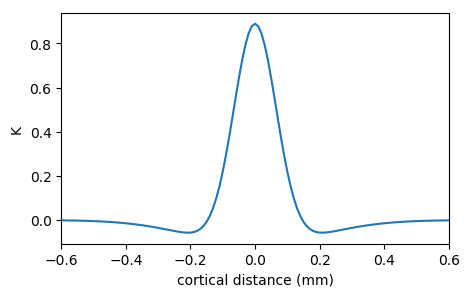
\includegraphics[width = 1.0\linewidth, trim={0 0 0 0}, clip=true]{figures/plot_K.png}
		\subcaption{$K_{aa'}$ where $a$ has been fixed a position $0$ and $a'$ varies from $-0.6$mm to $0.6$mm.}
		\label{fig:plotK}	
	\end{subfigure}%
	\hspace{0.1\linewidth}
	\begin{subfigure}[t]{0.38\linewidth}
		\centering
		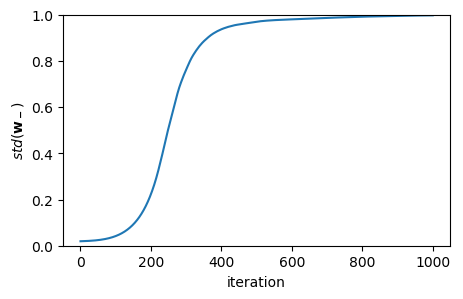
\includegraphics[width = 1.0\linewidth, trim={0 0 0 0}, clip=true]{figures/occsimtemp_stds.png}
		\subcaption{Standard deviation of ${\bf w}_-$ over time illustrating how ${\bf w}_-$ progresses from $\approx \bf 0$ to a vector of $ \pm 1$ after 800-1000 iterations.}
		\label{fig:stds}	
	\end{subfigure}%
\caption{}
\label{}
\end{figure}

We can also extract the vector ${\bf w}_-$ at different points in the simulation and plot the vector as a 1-dimensional heatmap along the x-direction where individual neurons are coloured from white to black according their ocular dominance (figure \ref{fig:occsim_int}).


\begin{figure}[h]
	\centering
	\begin{subfigure}[t]{0.49\linewidth}
		\centering
		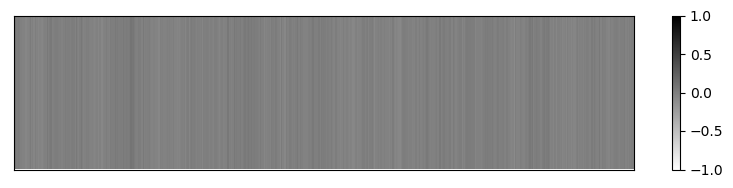
\includegraphics[width = 1.0\linewidth, trim={0 0 0 0}, clip=true]{figures/occsim_int/i50.png}
		%\subcaption{}
		%\label{fig:sim1vec}	
	\end{subfigure}%
	\hspace{0.01\linewidth}
	\begin{subfigure}[t]{0.49\linewidth}
		\centering
		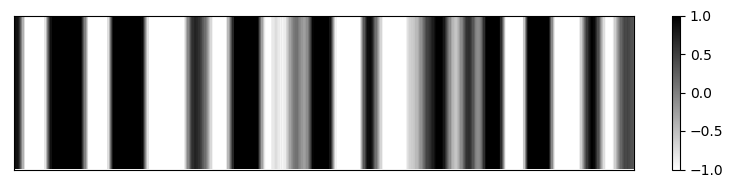
\includegraphics[width = 1.0\linewidth, trim={0 0 0 0}, clip=true]{figures/occsim_int/i300.png}
		%\subcaption{}
		%\label{fig:sim2vec}	
	\end{subfigure}%
	\hspace{0.01\linewidth}
	\begin{subfigure}[t]{0.49\linewidth}
		\centering
		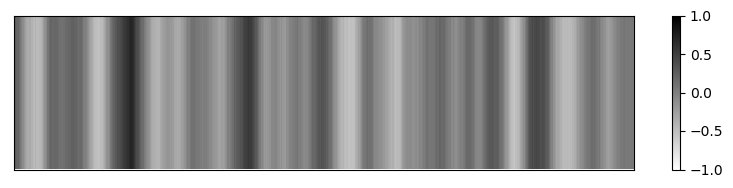
\includegraphics[width = 1.0\linewidth, trim={0 0 0 0}, clip=true]{figures/occsim_int/i200.png}
		%\subcaption{}
		%\label{fig:sim3vec}	
	\end{subfigure}%
	\hspace{0.01\linewidth}
	\begin{subfigure}[t]{0.49\linewidth}
		\centering
		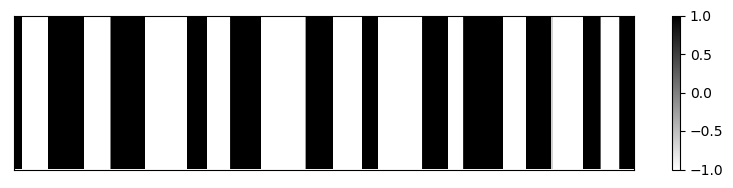
\includegraphics[width = 1.0\linewidth, trim={0 0 0 0}, clip=true]{figures/occsim_int/i1000.png}
		%\subcaption{}
		%\label{fig:sim3vec}	
	\end{subfigure}%
\caption{${\bf w}_-$ as a heatmap after 50, 200, 300 and 1000 iterations. We see that ocular dominance becomes increasingly strong over time and that the short-range excitation with long-range inhibition drives the formation of an oscillatory pattern of dominance.}
\label{fig:occsim_int}
\end{figure}

From our previous considerations, we expect the long-term behavior of ${\bf w}_-$ to be dominated by the prinpical eigenvector of $\bf K$.
In the case of periodic boundary conditions as imposed here, the eigenvectors of \textbf{K} are given by
\begin{equation}
e_a^\mu = \cos{(\dfrac{2 \pi \mu a}{512}-\phi)}
\end{equation}
Where the eigenvalues $\mu = \dfrac{512 \cdot d \cdot k}{2 \pi}$ take integer values given by the discrete fourier transform $\tilde K(\mu) $ of \textbf{K}.

Here, $k$ is the spatial frequency of the ocular dominance columns and $d$ is the separation between sites $a$ and $a+1$; $d = \dfrac{10 mm}{512}$. The principal eigenvector is thus the eigenfunction $e_\mu$ with $\mu$ corresponding to the maximum of $\tilde K(\mu)$.

To find the principal eigenvector of \textbf{K} and thus the expected long-term behavior of the system, we first find $\tilde K(k)$.
\begin{equation}
\tilde K (k) = \int_{-\infty}^\infty{K(x) e^{-2 \pi i k x} dx }
\end{equation}
We know that the fourier transform is a linear operator and that the fourier transform of a gaussian is given by
\begin{equation}
G(k) = \int_{-\infty}^\infty{ \dfrac{1}{\sqrt{2 \pi \sigma^2}} \, e^{\dfrac{-x^2}{2 \sigma^2}} e^{-2 \pi i k x} dx } 
= e^{\dfrac{-k^2 \sigma^2}{2}}
\end{equation}
This allows us to easily calculate the required fourier transform
\begin{equation}
\tilde K(k) = \sqrt{2 \pi \sigma^2} e^{ \dfrac{- k^2 \sigma^2}{2} } - \dfrac{1}{9} \sqrt{18 \pi \sigma^2 } e^{\dfrac{-9 k^2 \sigma^2}{2}}
\end{equation}
We plot this in figure \ref{fig:Ktilde} and find that the maximum of $\tilde K = 0.128$ occurs at $k = 8.17$. We can now find the value of $\mu$ corresponding to this maximum $\tilde K$ as
$
\mu_{max} = \dfrac{512 \,\,\, 8.17}{2 \pi} \dfrac{10}{512} = 13
$.

This allows us to calculate the principal eigenvector $e_{\mu_{max}}$ as a function of cortical distance and we plot this in figure \ref{fig:eigvec}. We note that the pattern of inhibition and excitation follows that of $K$ in figure \ref{fig:plotK}.
Since $\mu_{max}=13$, we expect to generate 13 periods of left and right dominance in a simulation which is consistent with the results in figure \ref{fig:occsim_int}. 

\begin{figure}[h]
	\centering
	\begin{subfigure}[t]{0.35\linewidth}
		\centering
		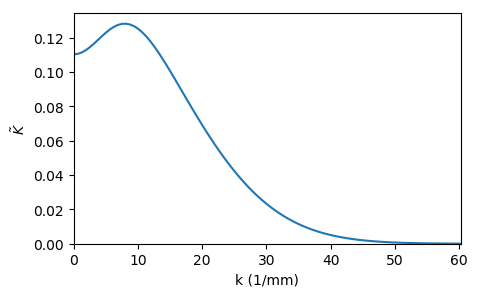
\includegraphics[width = 1.0\linewidth, trim={0 0 0 0}, clip=true]{figures/plot_Ktilde.png}
		\subcaption{Fourier transform of K as a function of spatial frequency $k$. This has a maximum of $k=8.17$ corresponding to $\mu=13$.}
		\label{fig:Ktilde}	
	\end{subfigure}%
	\hspace{0.1\linewidth}
	\begin{subfigure}[t]{0.35\linewidth}
		\centering
		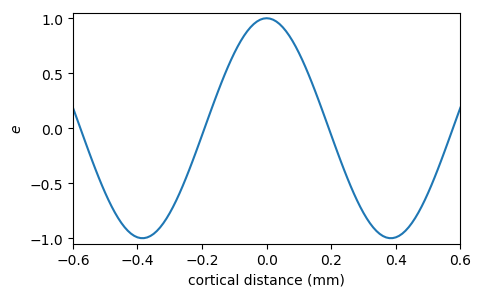
\includegraphics[width = 1.0\linewidth, trim={0 0 0 0}, clip=true]{figures/plot_eigvec.png}
		\subcaption{Principal eigenvector of K capturing the pattern of short-range excitation and long-range inhibition.}
		\label{fig:eigvec}	
	\end{subfigure}%
\caption{}
\label{}
\end{figure}

We now repeat our simulation of the system 1000 times and calculate the magnitude of the discrete fourier transform (DFT) at each trial. We plot the mean of the DFTs in figure \ref{fig:DFT} and see that the major components of our equilibrium ${\bf w}_-$ vector do indeed correspond to the values of $k$ for which $\tilde K$ is highest in figure \ref{fig:Ktilde}. 

\begin{figure}[h]
	\centering
	\begin{subfigure}[t]{0.35\linewidth}
		\centering
		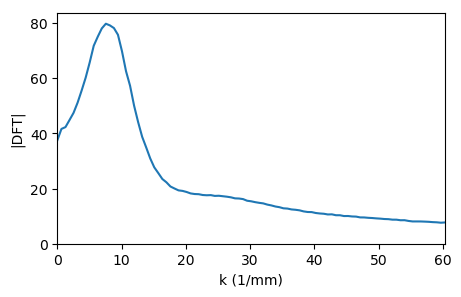
\includegraphics[width = 1.0\linewidth, trim={0 0 0 0}, clip=true]{figures/plot_DFT.png}
		\subcaption{Mean magnitude of the discrete fourier transform of the steady state ${\bf w}_-$ vector across 1000 simulations.}
		\label{fig:DFT}	
	\end{subfigure}%
	\hspace{0.1\linewidth}
	\begin{subfigure}[t]{0.35\linewidth}
		\centering
		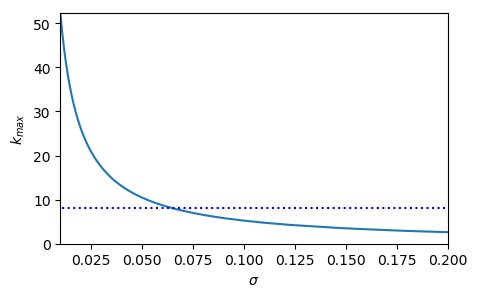
\includegraphics[width = 1.0\linewidth, trim={0 0 0 0}, clip=true]{figures/test_maxk.png}
		\subcaption{Principal eigenvector of \textbf{K}}
		\label{fig:maxk}	
	\end{subfigure}%
\caption{}
\label{}
\end{figure}

We find that the mean of the DFTs has a maximum of $79.7$ at $\mu = 13$ which is consistent with our analytical considerations suggesting that the largest component of the long-time ${\bf w}_-$ vector should correspond to the principal eigenvector which does indeed have $\mu = 13$

The stripe width in this model is determined by the spatial range of excitatory and inhibitory interactions which in turn is specified by the scale parameter $\sigma$ in equation \ref{eq:cortint}.
In order to decrease the stripe width in the model, we need to decrease the scale parameter $\sigma$ which leads to an increase in the value of $k$ that maximizes our discrete fourier transform and thus an increased frequency of the principal eigenvector of $\bf K$. In order to increase the stripe width, we instead increase $\sigma$.
The relationship between $\sigma$ and $k$ has been investigated numerically, and the value of $k$ that maximizes $\tilde K$ for a given $\sigma$ has been plotted in figure \ref{fig:maxk} which shows a rapid increase in frequency as $\sigma \rightarrow 0$.

To validate these results, we run two additional simulations; one with $\sigma = 0.012$ for which we expect $k=40.31$ and thus $\mu = 69$, and one with $\sigma=0.174$ for which we expect $k=3.01$ and $\mu = 5$. We plot the resulting steady state ${\bf w}_-$ vectors in figure \ref{fig:sigs} and see that we do indeed get increasingly wider stripes with increasing $\sigma$ and that the number of full periods matches the expected value of $\mu$.

\begin{figure}[h]
	\centering
	\begin{subfigure}[t]{0.60\linewidth}
		\centering
		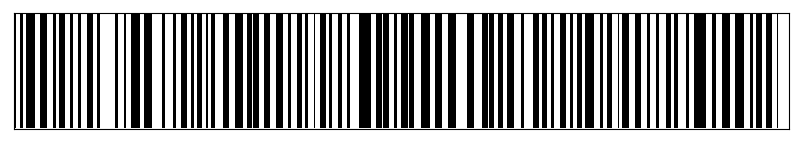
\includegraphics[width = 1.0\linewidth, trim={0 0 0 0}, clip=true]{figures/occsim_012_heat.png}
		\subcaption{$\sigma = 0.012$ giving $k=40.31$ and $\mu = 69$}
		%\label{fig:sim1vec}	
	\end{subfigure}%
	\hspace{0.03\linewidth}
	\begin{subfigure}[t]{0.60\linewidth}
		\centering
		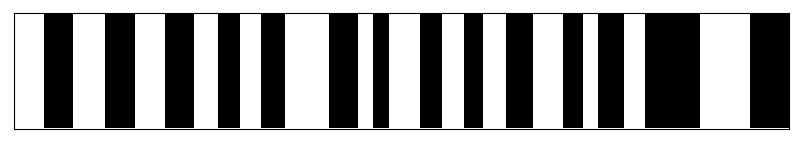
\includegraphics[width = 1.0\linewidth, trim={0 0 0 0}, clip=true]{figures/occsim_066_heat.png}
		\subcaption{$\sigma = 0.066$ giving $k=8.17$ and $\mu = 13$}
		%\label{fig:sim2vec}	
	\end{subfigure}%
	\hspace{0.03\linewidth}
	\begin{subfigure}[t]{0.60\linewidth}
		\centering
		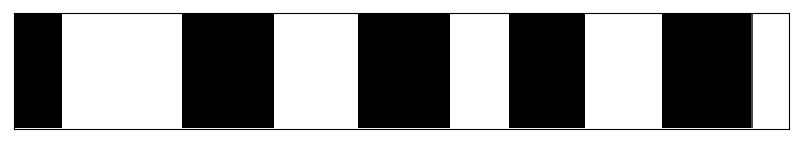
\includegraphics[width = 1.0\linewidth, trim={0 0 0 0}, clip=true]{figures/occsim_174_heat.png}
		\subcaption{$\sigma=0.174$ giving $k=3.01$ and $\mu = 5$}
		%\label{fig:sim3vec}	
	\end{subfigure}%
\caption{Simulations of the ocular dominance system for different values of $\sigma$ corresponding to different interaction ranges. Longer-range interactions lead to wider stripes.}
\label{fig:sigs}
\end{figure}

We could of course also alter the cortical interactions in other ways, e.g. by altering the ratio of the two gaussians from $1 : 1/9$ or by changing the relative standard deviations from $\sigma_2 = 3 \sigma_1$, but these options are not explored further as they do not preserve the form of the interactions.

\section{The elastic net}

The Travelling salesman problem is an example of an NP complete problem, and there is thus no (current) algorithm that can solve it in polynomial time. As the number of nodes to be visited N increases, we are therefore forced to use various heuristic algorithms to try to approximate optimal solutions. One such algorithm dubbed the 'elastic net' was proposed by Durbin and Willshaw in a 1987 \textit{letter to Nature}.

In this algorithm, there are N cities to be visited, and this is achieved by distorting an initial path of M points until it runs through all N cities in a way that locally minimizes the path length L.
We denote the cities to be visited $\{x_i\}$ and the M points on the path travelled on $\{y_j\}$. At each timepoint the elastic net then updates each point on the path according to
\begin{equation}\label{eq:update}
\Delta y_j =\alpha \sum_i{w_{ij}(x_i-y_j) + \beta K (y_{j+1} - 2y_j + y_{j-1})} 
\end{equation}
The first term serves to decrease the distance between a point on the path and a city, ensuring that all points on the path will eventually run through a city. The second term serves to bring the points as close to each other as possible, ensuring that the path length is minimized.

In equation \ref{eq:update}, the weights $w_{ij}$ are given by
\begin{equation}
w_{ij} = \dfrac{\phi(|x_i-y_j|, K)}{\sum_k{\phi(|x_i-y_k|, K)}}
; ~~~
\phi (d, K) = \exp{(\dfrac{-d^2}{2K^2})}
\end{equation}
This implementation of the elastic net corresponds to minimizing an energy function
\begin{equation}\label{eq:energy}
E = -\alpha K (\sum_i{\ln{\sum_j{\phi(|x_i-y_j|, K)}}})+\beta \sum_j{|y_{j+1}-y_j|^2}
\end{equation}
Where again the first term penalizes when the path is far from a city and the second term penalizes a long path.
Our update step from equation \ref{eq:update} then has the property
$
\Delta y_j = -K \dfrac{\partial E}{\partial y_j}
$.

We are thus carrying out gradient descent on equation \ref{eq:energy} with adaptive learning rate K, ensuring that we will eventually arrive at a local minimum of the energy.

Over the course of the optimization, Durbin and Willshaw reduce K by 1\% every 25 iterations from $K=0.2$ to $K=0.01$ and fix $M = 2.5N$. However, given the advances in computing power since 1987, we can explore the effect of K and M on the performance of the algorithm more thoroughly.

For the remainder of this section we set $\alpha = 0.2$ and $\beta = 2.0$ as in Durbin and Willshaw, and we choose points on our initial path to be evenly spread out at a distance $0.1+\text{unif}(-0.001, 0.001)$ from the centroid of the cities. Cities are generated as a grid of 100 randomly distributed points in a 1x1 square.

We let K decay exponentially according to $K = 0.2*\exp{(-\lambda n)}$ where n is the number of timesteps, and a simulation is considered finished when $K < 0.001$. We can now vary lambda and the number of points M on our path to optimize the elastic net. The result of a coarse-grained parameter search is given in figure \ref{fig:tspopt}.  

\begin{figure}[h]
	\centering
	\begin{subfigure}[t]{0.35\linewidth}
		\centering
		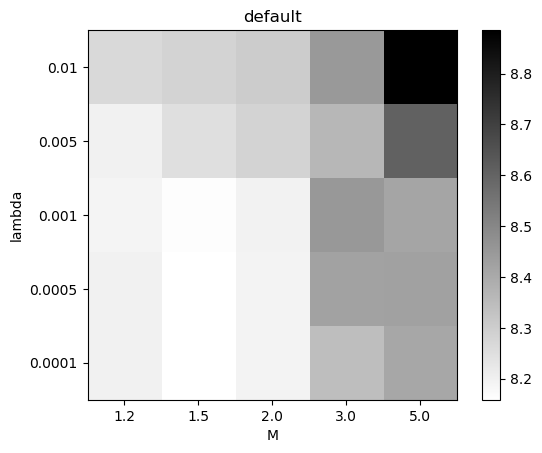
\includegraphics[width = 1.0\linewidth, trim={8 10 7 20}, clip=true]{figures/Ls.png}
		\subcaption{Length of final path}
		\label{fig:Ls}	
	\end{subfigure}%
	\hspace{0.1\linewidth}
	\begin{subfigure}[t]{0.35\linewidth}
		\centering
		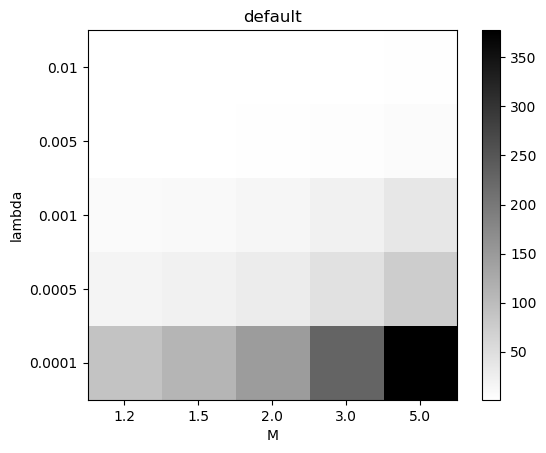
\includegraphics[width = 1.0\linewidth, trim={8 10 7 20}, clip=true]{figures/Ts.png}
		\subcaption{Time to convergence (seconds)}
		\label{fig:Ts}	
	\end{subfigure}%
\caption{Performance (left) and computational time (right) for the elastic net approach to the travelling salesman problem as a function of decay rate $\lambda$ and number of points on the path M. All simulations were run on the same set of 100 cities with remaining parameters as specified in the main text.}
\label{fig:tspopt}
\end{figure}

We see from figure \ref{fig:Ls} that in contrast to the parameters used by Durbin and Willshaw, we achieve the best performance with a relatively small value of M=1.5N since small values of M tend to reduce the popensity of the system to get caught in higher-energy local minima compared to $M > 2N$. We also note that there is an increase in performance with decreasing lambda as expected, but this effect is neglible for $\lambda < 0.0005$.

From figure \ref{fig:Ts} we see that the time taken for a simulation is approximately linear in both $\lambda$ and M. Considering this data together with figure \ref{fig:Ls}, we fix M=1.5 and $\lambda = 0.0005$ for the remainder of our simulations. A more finegrained optimization could be carried out, but this was not deemed particularly informative since the details of the optimization will depend upon the specific grid being investigated. However, the above analysis was repeated with two additional random grids and similar patterns were observed.

We can now investigate how the path develops as K decreases for our optimum parameters of M=1.5 and $\lambda = 0.0005$ (figure \ref{fig:tspsim}). We see that the path initially expands relatively uniformly to decrease the distance from the far-away cities to the path. The path then locally distorts as it moves closer to every individual point. This is finally achieved at K=0.001 where the path has converged and the salesman visits every city. When M gets too close to N, the algorithm occasionally converges to a local minimum where the path does not visit every city. For $M \geq 1.5N$ this has not been observed.

\begin{figure}[h]
	\centering
	\begin{subfigure}[t]{0.24\linewidth}
		\centering
		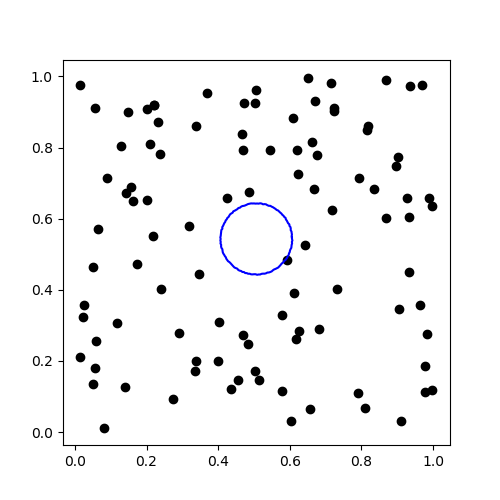
\includegraphics[width = 1.0\linewidth, trim={20 20 30 30}, clip=true]{figures/optimum_1.png}
		\subcaption{K=0.2}
		\label{fig:sim1}	
	\end{subfigure}%
	%\hspace{0.01\linewidth}
	\begin{subfigure}[t]{0.24\linewidth}
		\centering
		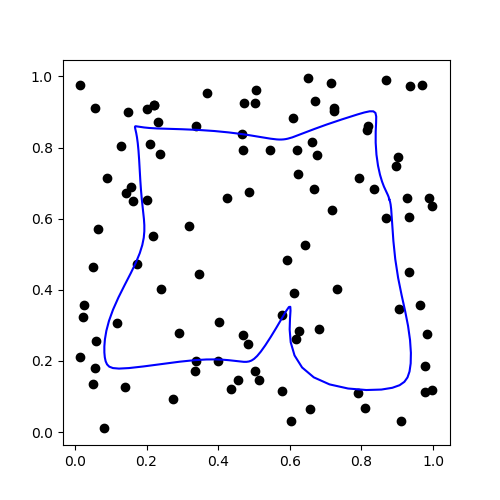
\includegraphics[width = 1.0\linewidth, trim={20 20 30 30}, clip=true]{figures/int/optimum_K6_011.png}
		\subcaption{K=0.11}
		\label{fig:sim2}	
	\end{subfigure}%
	%\hspace{0.01\linewidth}
	\begin{subfigure}[t]{0.24\linewidth}
		\centering
		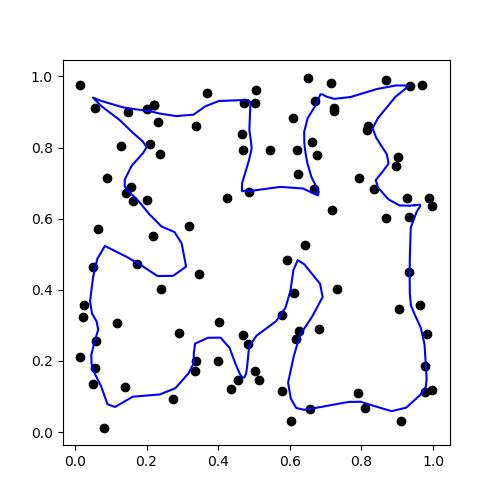
\includegraphics[width = 1.0\linewidth, trim={20 20 30 30}, clip=true]{figures/int/optimum_K16_004.png}
		\subcaption{K=0.04}
		\label{fig:sim3}	
	\end{subfigure}%
	%\hspace{0.01\linewidth}
	\begin{subfigure}[t]{0.24\linewidth}
		\centering
		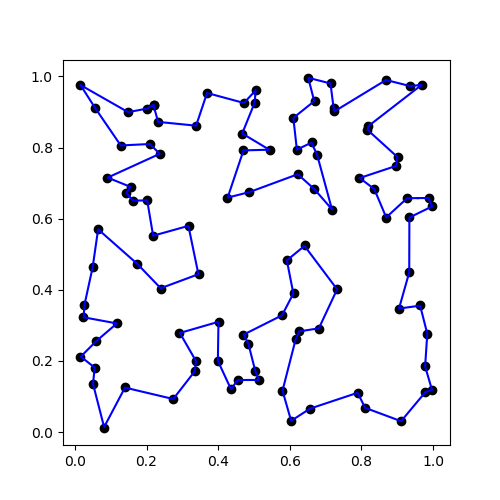
\includegraphics[width = 1.0\linewidth, trim={20 20 30 30}, clip=true]{figures/optimum_2.png}
		\subcaption{K=0.001}
		\label{fig:sim4}	
	\end{subfigure}%
\caption{Timecourse of the travelling salesman simulation with M=1.5 and $\lambda = 0.0005$}
\label{fig:tspsim}
\end{figure}

At a first glance, this looks like a reasonable route as there are no obvious detours or crossovers. However, to get a better idea of how efficient the elastic net method is, we can compare it to the well established travelling salesman method of simulated annealing. For this comparison, we implement simulated annealing as described in \textit{Stochastic Processes} (Chang 2007).

We can consider a given TSP route (order of cities) to be a point in a set $\mathcal{S}$ of $\dfrac{(n-1)!}{2}$ possible routes. Our aim is to find a route that minimizes the total length $L$ by moving between neighboring points on $\mathcal{S}$. Here, we define 'neighboring points' as routes that can be interconverted by reversing the part of the path between two cities.

In the simulated annealing algorithm, one iteration involves moving uniformly at random to a neighboring point in $\mathcal{S}$ and calculating the length $L1$ of the new route obtained.
If $L1 < L0$, we accept this new route as our current route.
If $L1 > L0$, we accept the new route with probability $p = \exp{(-\dfrac{L1-L0}{T})}$. Otherwise we retain the old route.

This finite probability of accepting a worse route allows us to move out of local minima and thus to approach the global minimum with a higher probability than a simple gradient descent algorithm. This is similar to e.g. the annealing process in glass (from which the algorithm has its name), or protein folding in a cell where the finite temperature allows for stochastic movement out of local minima in conformational space.\\
Over the course of the simulation, we decrease the tempeature according to
$
T_n = \dfrac{T_0}{ln(n)}
$.
Here n is the number of iterations. The decrease in temperature makes it increasingly unlikely that we will move to a worse route, and in the limit of $T \rightarrow 0$, we will move to the nearest local minimum as there is no thermal energy in the system to drive it to a longer path.

Setting $T_0=10$ and running $10^7$ iterations has been found empirically to give good results on a timescale similar to the one observed for the elastic net ($\approx$ 20 seconds).
To compare the two methods, we use the map of 100 cities considered above as well as two new randomly generated maps. We then quantify the optimum route generated by the elastic net in terms of both route length and time to convergence. We compare this to 30 trials of simulated annealing since the simulated annealing process is stochastic and results thus vary per trial. A summary of the results is given in table \ref{tab:tsp}.

\begin{table}[h]
\centering
\begin{tabular}{ |c|c|c|c|}
\hline
 &Map 1 &Map 2 & Map 3 \\
\hline
Elastic net & 8.159 & 7.771 & 7.815 \\
Time (s) & 23.32 & 23.819& 24.91 \\
\hline
Simulated annealing & 7.956 (0.047) & 7.768 (0.052)& 7.633 (0.075)\\
Time (s) & 19.06 (1.33) & 19.47 (1.97) & 18.47 (1.12)\\
\hline
\end{tabular}
\caption{Performance and computational time for the elastic net and simulated annealing across three different maps of 100 randomly generated cities. For simulated annealing, results are reported as mean (std).}
\label{tab:tsp}
\end{table}

We see that simulated annealing consistently outperforms the elastic net, both in terms of the converged route and the time taken to find this route. This can be seen qualitatively in figure \ref{fig:comp1}.

\begin{figure}[h]
	\centering
	\begin{subfigure}[t]{0.28\linewidth}
		\centering
		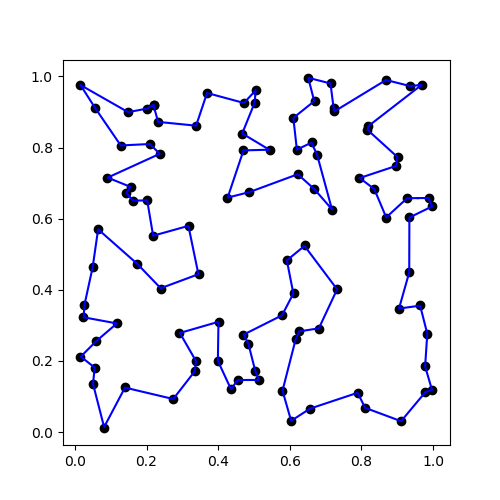
\includegraphics[width = 1.0\linewidth, trim={20 20 30 30}, clip=true]{figures/optimum_2.png}
		\subcaption{Elastic net (L=8.159)}
		\label{fig:comp1el}	
	\end{subfigure}%
	\hspace{0.1\linewidth}
	\begin{subfigure}[t]{0.28\linewidth}
		\centering
		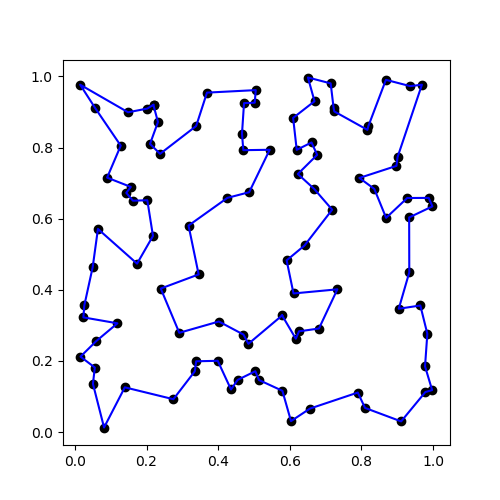
\includegraphics[width = 1.0\linewidth, trim={20 20 30 30}, clip=true]{figures/orig_citiesmin.png}
		\subcaption{Simulated annealing (L = 7.919)}
		\label{fig:comp1an}	
	\end{subfigure}%
\caption{Optimum routes for map 1 found by the elastic net method and simulated annealing. Simulated annealing finds a shorter route than the elastic net, and this route involves only visiting the inner region of the map once. }
\label{fig:comp1}
\end{figure}

However, for map 2 simulated annealing only slightly outperforms the elastic net on average and performs worse in almost half the trials, raising the question of whether there are any profound insights to be gained from this difference between maps. For map 1, we find that the optimum route from simulated annealing appears very asymmetric. It is thus less likely to be converged upon by the elastic net, the dynamics of which lead to an initial expansion of the route followed by the formation of local invaginations (figure \ref{fig:tspsim}).

For map 2, on the contrary, the optimum route from simulated annealing appears more symmetrical which might explain why the elastic net comes close to the performance of simulated annealing in this case.


\begin{figure}[h]
	%\hspace{0.31\linewidth}
	\centering
	\begin{subfigure}[t]{0.28\linewidth}
		\centering
		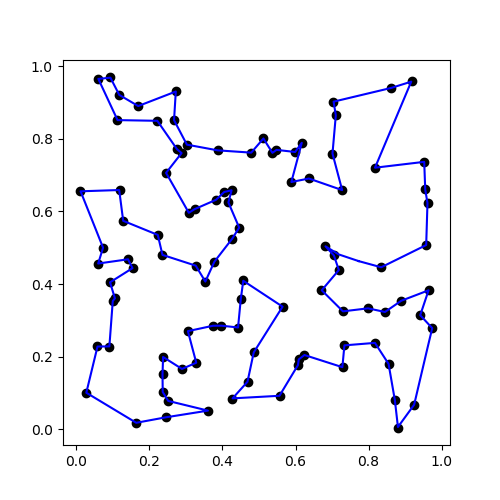
\includegraphics[width = 1.0\linewidth, trim={20 20 30 30}, clip=true]{figures/rand1_2.png}
		\subcaption{Elastic net (L = 7.771)}
		\label{fig:comp2el}	
	\end{subfigure}%
	\hspace{0.1\linewidth}
	\begin{subfigure}[t]{0.28\linewidth}
		\centering
		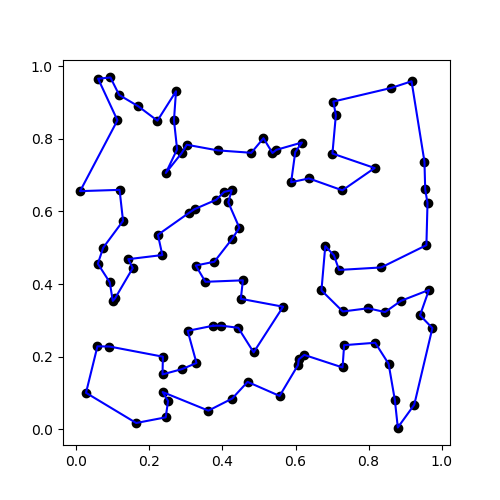
\includegraphics[width = 1.0\linewidth, trim={20 20 30 30}, clip=true]{figures/rand1_citiesmin.png}
		\subcaption{Simulated annealing (L = 7.685)}
		\label{fig:comp2an}	
	\end{subfigure}%
\caption{For map 2, the optimum solution found by simulated annealing is more symmetrical, and the elastic net comes close to the performance of simulated annealing.}
\label{fig:comp2}
\end{figure}


Simulated annealing is thus a superior method to the elastic net in terms of solving the travelling salesman problem, but we see that the elastic net still produces reasonable routes that are comparable in length to those generated by simulated annealing albeit generally more symmetric. The elastic net methodology is however still interesting due to its dynamics and general applicability to problems involving mappings between different topologies.

As an example, we use the elastic net to model ocular dominance in two dimensions, inspired by Goodhill and Willshaw (1989). We imagine the 'tour' as being a plane representing a region of the visual cortex where each point has elastic connections to its four neighboring points. The retinal inputs are represented by two horizontal planes corresponding to the left and right eyes respectively with each point being the equivalent of a city in the TSP. We now index our cortical plane by $i, j$ and the retinal positions by $a, b$. This gives rise to a modified update step:
\begin{equation}\label{eq:update2}
\Delta y_{ij} =\alpha \sum_{a,b}{w_{ab,ij}(x_{ab}-y_{ij})} + \beta K (y_{i \, j+1} + y_{i+1 \, j} - 4y_{i \, j} + y_{i \, j-1} + y_{i-1 \, j})
\end{equation}
The weights $w_{ab,ij}$ are given by Gaussians of Euclidean distances as before. The degree of correlation between left and right eyes are defined by the distance $2l$ between the two ocular planes and the inter-point separation $2d$ determines the separation of photoreceptors.

The stripe width of the emerging pattern is governed by the ratio $l/d$. As $l/d$ increases, cortical-cortical correlation becomes stronger relative to retinal correlation, leading to broader stripes. As $l/d$ decreases, the opposite trend is observed.

This is illustrated in figure \ref{fig:widths} where we reproduce the result of Goodhill and Willshaw (1989) showing the effect of $l/d$ on stripe width. We fix $2d=0.05$ and let $l$ be equal to 0.050 (figure \ref{fig:dom05}), 0.075 (figure \ref{fig:dom075}) and 0.100 (figure \ref{fig:dom100}) leading to successive increases in stripe width. For these simulations we fix $N=20$ and $M=40$ where $N$ and $M$ are the squareroots of the number of retinal and cortical points respectively.

\begin{figure}[h]
	%\hspace{0.31\linewidth}
	\centering
	\begin{subfigure}[t]{0.23\linewidth}
		\centering
		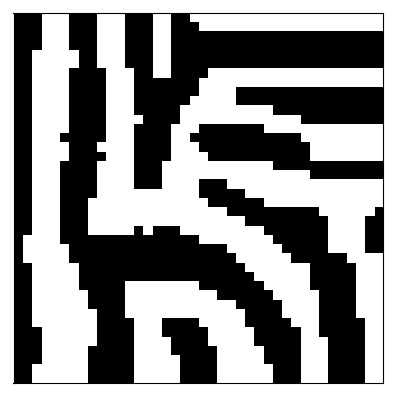
\includegraphics[width = 1.0\linewidth, trim={5 5 5 10}, clip=true]{figures/N20M40l05d05_2_dominance.png}
		\subcaption{$l = 0.050$; $2d = 0.05$}
		\label{fig:dom05}	
	\end{subfigure}%
	\hspace{0.03\linewidth}
	\begin{subfigure}[t]{0.23\linewidth}
		\centering
		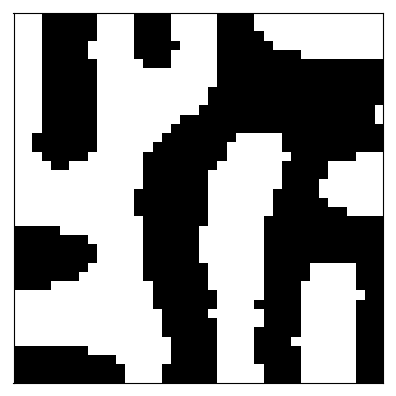
\includegraphics[width = 1.0\linewidth, trim={5 5 5 10}, clip=true]{figures/N20M40l075d05_2_dominance.png}
		\subcaption{$l = 0.075$; $2d = 0.05$}
		\label{fig:dom075}	
	\end{subfigure}%
		\hspace{0.03\linewidth}
	\begin{subfigure}[t]{0.23\linewidth}
		\centering
		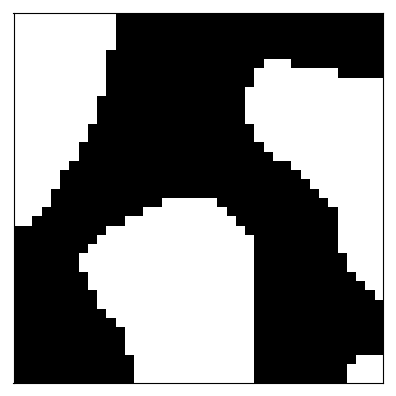
\includegraphics[width = 1.0\linewidth, trim={5 5 5 10}, clip=true]{figures/N20M40l100d05_2_dominance.png}
		\subcaption{$l = 0.100$; $2d = 0.05$}
		\label{fig:dom100}	
	\end{subfigure}%
\caption{Ocular dominance maps resulting from a two-dimensional elastic net simulation. Individual squares (cortical neurons) are coloured according to whether they are most closely associated with the right (white) or left (black) retina. Stripe width increases with $l/d$.}
\label{fig:widths}
\end{figure}

For the purpose of these simulations, cortical points were initialized uniformly at random in the xy plane corresponding to random initial retinal-cortical connectivity. The z locations of the points were generated uniformly at random between $\pm 0.01$ corresponding to balanced but noisy ocular input.

Interestingly, we see from figure \ref{fig:xs_075} that in addition to the emergence of ocular dominance, this simulation also leads to the emergence of visual cortical maps as has been observed experimentally. From our initial random connectivity, we see that at the end of the simulation, cortical neurons with large y-values receive input from retinal neurons with small x-values (white) and vice versa. Similarly, neurons with small x-values in the cortex receive input from retinal neurons with small y-values and vice versa (not shown). This swap of the x and y axes between the retinal and cortical coordinate systems may at first seem surprising, but since our energy landscape has $D_{4h}$ symmetry, this is entirely equivalent to an $x \rightarrow x$ and $y \rightarrow y$ mapping.

\begin{figure}[h]
	%\hspace{0.31\linewidth}
	\centering
	\begin{subfigure}[t]{0.20\linewidth}
		\centering
		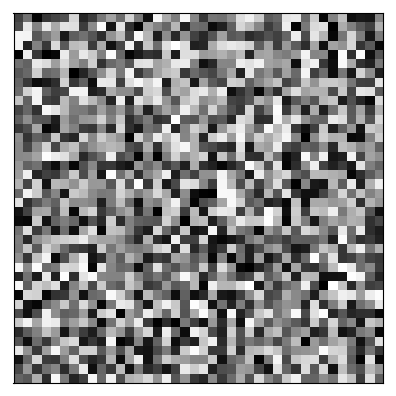
\includegraphics[width = 1.0\linewidth, trim={5 5 5 10}, clip=true]{figures/N20M40l075d05_1_xvals.png}
		%\subcaption{l = 0.075, 2d = 0.05}
		%\label{fig:x075_1}	
	\end{subfigure}%
	\hspace{0.15\linewidth}
	\begin{subfigure}[t]{0.20\linewidth}
		\centering
		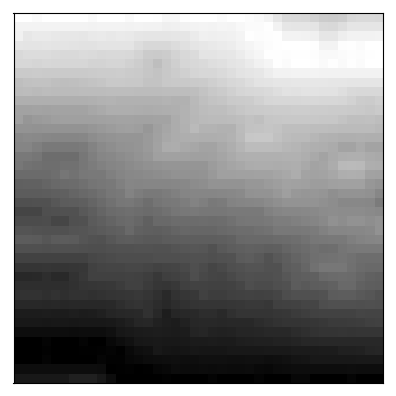
\includegraphics[width = 1.0\linewidth, trim={5 5 5 10}, clip=true]{figures/N20M40l075d05_2_xvals.png}
		%\subcaption{Simulated annealing (L = 7.685)}
		%\label{fig:x075_2}	
	\end{subfigure}%
\caption{Retinal-to-cortical mapping in the retinal x direction at the beginning (left) and end (right) of a simulation with $l = 0.075$ and $2d = 0.05$. x and y axes correspond to locations in the cortex. Colours indicate retinal connectivity (i.e. location in retinal space) with white and black regions corresponding to cortical neurons with input from retinal neurons with low and high x-values respectively. We see that neurons self-organize from the random initial connectivity to generate a cortical map.}
\label{fig:xs_075}
\end{figure}




\section{Cart pole balancing problem}

The Cart Pole Balancing Problem is a commonly used task in machine learning and computational neuroscience to assess the performance and adaptability of a network. We solve this task using a network described by Barto et al (1983). This network consists of only two elements: an
\textit{Associate Search Element} (ASE) which picks a decision based on a reward signal and eligibility trace, and an
\textit{Adaptive Critic Element} (ACE) which provides the ASE with a predicted reward over continuous time rather than a discrete reward at the end of a trial.

The state of the cartpole system is defined by a vector $(x, \theta, \dot x, \dot \theta)$ where $x$ is the position of the cart on a one-dimensional track with $x \in [-2.4, 2.4]$,
$\theta$ is the angle of the pole from vertical and dots represent time derivatives. A trial is considered to have failed when $|x| \geq 2.4$ or $| \theta | \geq 12 \degree$.
We divide the state space into 162 distinct regions defined by\\
$x \in [-2.4,-0.8], [-0.8,0.8],[0.8,2.4]$ (m)\\
$\theta \in [-12,-6],[-6,-1],[-1,0],[0,1],[1,6],[6,12]$ ($\degree$)\\
$\dot x \in [-\infty,-0.5],[-0.5,0.5],[0.5,\infty]$ (m/s)\\
$\dot \theta \in [-\infty,-50],[-50,50],[50,\infty]$ ($\degree$/s)

At any time t, the system will be in a given state $state(t)$ and it receives an impulse $y(t)$ either to the right or to the left depending on the relative predicted reward for right- and left-wards impulses. We therefore map a given state vector to a binary 162-dimensional vector $x$ that has all elements equal to zero except for the element corresponding to the current state of the system, and let the impulse at time $t$ be given by equation \ref{eq:impulse}.
\begin{equation}\label{eq:impulse}
y(t) = \text{sign}[\sum_i^{162}{w_i(t)x_i(t)} + \mathcal{N}(0, \sigma^2)] = \text{sign}[w_{state(t)}(t) + \mathcal{N}(0, \sigma^2)] 
\end{equation}
Where $x_i(t)$ is $1$ if the system is in state $i$ at time $t$ and zero otherwise, and $w_{state(t)}(t)$ is the weight at time t corresponding to the state of the system at time t. The Gaussian noise both simulates noise in real neural systems and allows our cart pole balancing system to explore the available state space.

For this ASE we update the weights according to
\begin{equation}
w_i(t+1) = w_i(t) + \alpha r(t) e_i(t)
\end{equation}
This is a three-factor learning rule where $\alpha$ is the learning rate, $r(t)$ is the global reward at time $t$ and $e_i(t)$ is the eligibility trace of unit $i$ at time $t$. For the pole balancing problem, $r=0$ throughout a trial and becomes $1$ when failure occurs. We update the eligiblity traces according to
\begin{equation}
e_i(t+1) = \delta e_i(t) + (1-\delta) y(t) x_i(t)
\end{equation}
where $\delta$ determines the trace decay rate and $x, y$ are as defined above.

The ASE on its own does not perform particularly well given the sparse error signal which only occurs after a long sequence of events. Performance is better if we include an ACE which estimates a predicted reward at all times.
The predicted reward is given by
\begin{equation}
\hat r(t) = r(t) + \gamma p(t) - p(t-1)
\end{equation}
Here, $\gamma$ leads to the predicted reward tending towards 0 in the case of prolonged periods without external reinforcement.
$p(t)$ is a prediction of eventual reinforcement, given by
\begin{equation}
p(t) = \sum_i^{162}{v_i(t)x_i(t) = v_{state(t)}(t)}
\end{equation}
This requires us to update the weights $v_i$ such that they remain an accurate predictor of reward. This is achieved using the learning rule
\begin{equation}
v_i(t+1) = v_i(t) + \beta[r(t) + \gamma p(t) - p(t-1)] \bar x_i(t)
\end{equation}
Here, $\beta$ determines the learning rate and $r(t)$ is the external reinforcement signal as above. $\bar x_i(t)$ is similar to the eligibility trace $e_i(t)$ for the ASE and is updated according to
\begin{equation}
\bar x_i(t+1) = \lambda \bar x_i(t) + (1-\lambda)x_i(t) 
\end{equation}
Where $\lambda$ is the trace decay rate. This is equivalent to the update rule for $e_i(t)$ in the case where $y_i(t) = 1$.


We initialize all $e_i, w_i, v_i, \bar x_i = 0$ at time $t=0$.
We intialize the cart at x=0 and the pole at an angle of 0 degrees.
We then integrate the above equations using Euler integration with a timestep of 0.02 as in Barto et al. and similarly let the parameters of the system be given by $~$
$\alpha = 1000$,
$\beta = 0.5$,
$\delta = 0.9$,
$\gamma = 0.95$,
$\lambda = 0.80$,
$\sigma = 0.01$.

Using these parameters, the system learns the balancing task in 20-80 trials and we show the result of the first 1000 seconds of simulated time in an example simulation in figure \ref{fig:balance_example}.

\begin{figure}[h]
	\centering
	\begin{subfigure}[t]{0.28\linewidth}
		\centering
		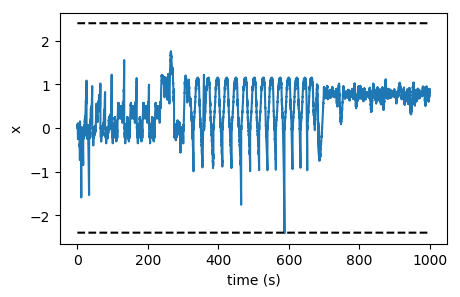
\includegraphics[width = 1.0\linewidth, trim={0 0 0 0}, clip=true]{figures/learn50000_xs.png}
		%\subcaption{Elastic net (L=8.159)}
		%\label{fig:comp1el}	
	\end{subfigure}%
	\hspace{0.1\linewidth}
	\begin{subfigure}[t]{0.28\linewidth}
		\centering
		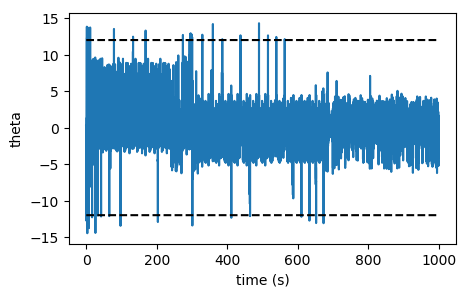
\includegraphics[width = 1.0\linewidth, trim={0 0 0 0}, clip=true]{figures/learn50000_thetas.png}
		%\subcaption{Simulated annealing (L = 7.919)}
		%\label{fig:comp1an}	
	\end{subfigure}%
\caption{Cart pole balancing simulation showing x (left) and theta (right) over 1000 seconds of simulated time.}
\label{fig:balance_example}
\end{figure}

We see that the system more commonly fails due to the pole falling than due to the cart exiting the arena. However, these two variables are correlated so we expect learning in one parameter to also help performance in the other.
This is illustrated in figure \ref{fig:earlycart} where we see that in many cases where the poll falls, the cart is also gaining momentum.

Over the course of the simulation we expect the system to learn that states with high $\theta$ and high $\dot \theta$ have low predicted reward as they will likely lead to system failure, and similarly for states with very negative $\theta$ and $\dot \theta$. To verify this, we plot the value of $v$ as a function of $\theta$ and $\dot \theta$ averaged over $x$ and $\dot x$ in figure \ref{fig:learned} after 100,000 seconds of simulated time.


\begin{figure}[h]
	\centering
	\begin{subfigure}[t]{0.32\linewidth}
		\centering
		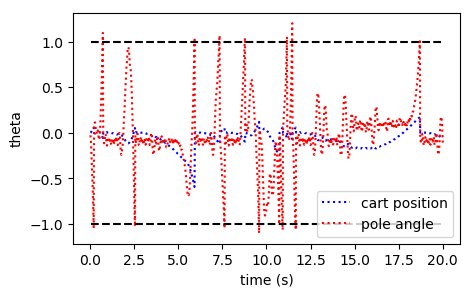
\includegraphics[width = 1.0\linewidth, trim={0 0 0 5}, clip=true]{figures/learn1000_xs_thetas.png}
		\subcaption{Cart position x and pole angle $\theta$ for the first 20 seconds of an example simulation.}
		\label{fig:earlycart}	
	\end{subfigure}%
	\hspace{0.1\linewidth}
	\begin{subfigure}[t]{0.34\linewidth}
		\centering
		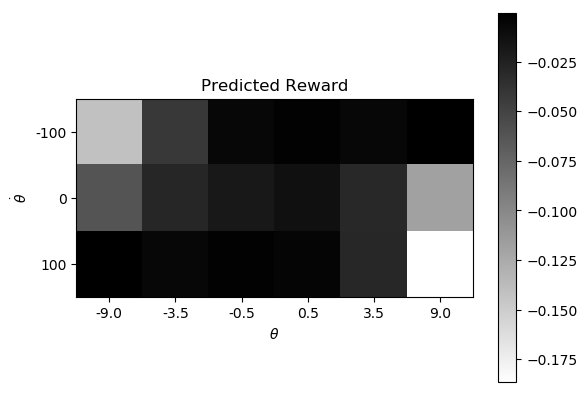
\includegraphics[width = 1.0\linewidth, trim={10 40 80 70}, clip=true]{figures/learnvs_vs.png}
		\subcaption{$v$ averaged over $x$ and $\dot x$ as an indication of expected reward for different combinations of $\theta$ and $\dot \theta$.}
		\label{fig:learned}	
	\end{subfigure}
\caption{}
\label{fig:balancing}
\end{figure}

We see that these extreme states do indeed have a low predicted reward and that $v$ has a 'ridge' of states with high predicted reward running from the lower left to the upper right corner.

To investigate the rate of learning, we follow the example of Barto et al. and run the network for 500,000 iterations corresponding to 100,000 seconds of simulated time. We then quantify the length of each trial with a trial terminating once the system fails. After each trial, we reset all eligibility traces $e$ to 0. We then plot the trial length against trial number for a single simulation (\ref{fig:singletrial}) or as an average over 500 simulations (\ref{fig:500trials}).

\begin{figure}[h]
	\centering
	\begin{subfigure}[t]{0.28\linewidth}
		\centering
		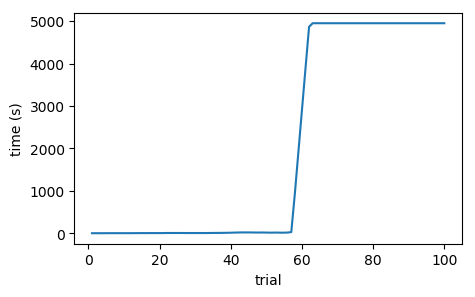
\includegraphics[width = 1.0\linewidth, trim={0 0 0 0}, clip=true]{figures/learn500000_performance.png}
		\subcaption{Performance for a single example trial.}
		\label{fig:singletrial}	
	\end{subfigure}%
	\hspace{0.1\linewidth}
	\begin{subfigure}[t]{0.28\linewidth}
		\centering
		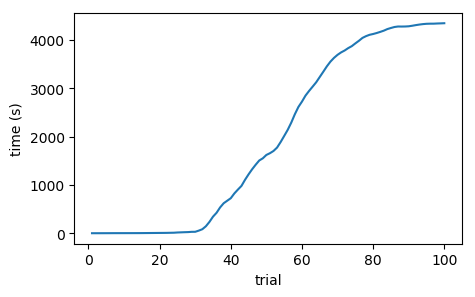
\includegraphics[width = 1.0\linewidth, trim={0 0 0 0}, clip=true]{figures/real_meanperformance.png}
		\subcaption{Mean performance over 500 trials.}
		\label{fig:500trials}	
	\end{subfigure}
\caption{Plots of trial duration (simulated time) against trial number. We see that for a single trial, there is a very steep increase in trial duration after the final failure and over 500 trials this averages out to approximately linear learning between trial 30 and 70. By 100 trials, there are generally no more failures.}
\label{fig:cartpole_learning}
\end{figure}

Having investigated the rate of learning for the parameters used in Barto et al., we proceed to investigate the effect of some of the key parameters on the learning rate. For the purpose of these investigations, we consider the system to have learned when the mean learning curve of the system over 100 simulations exceeds 10\% of the total simulation time; i.e. when the mean trial length exceeds 1000 seconds of simulated time. We then average this performance over 10 sets of simulations and calculate this metric for a range of different parameters in figure \ref{fig:params}.

\begin{figure}[h]
	\centering
	\begin{subfigure}[t]{0.28\linewidth}
		\centering
		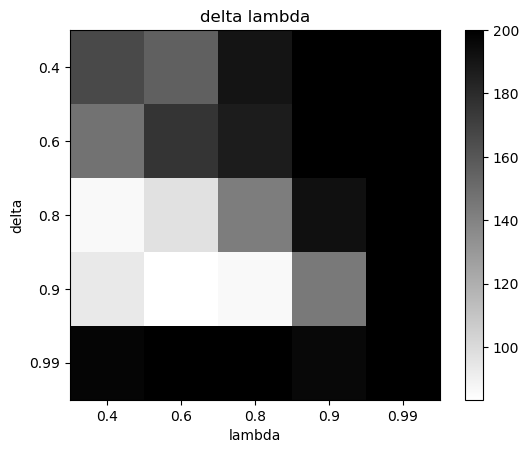
\includegraphics[width = 1.0\linewidth, trim={0 0 0 0}, clip=true]{figures/real_delta_lambda_heat.png}
		\subcaption{Performance for different eligibility trace decay rates $\delta$ and $\lambda$}
		\label{fig:delta_lambda}	
	\end{subfigure}%
	\hspace{0.05\linewidth}
	\begin{subfigure}[t]{0.28\linewidth}
		\centering
		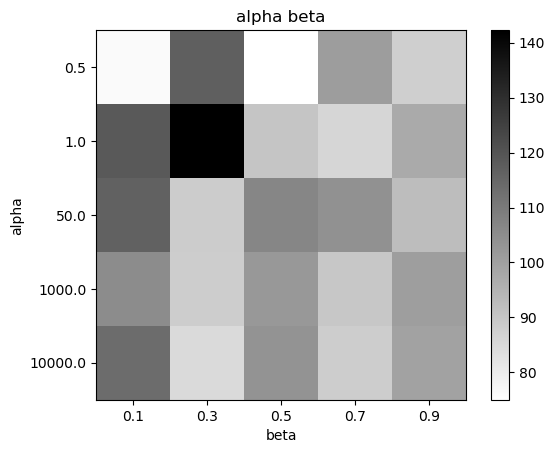
\includegraphics[width = 1.0\linewidth, trim={0 0 0 0}, clip=true]{figures/test_alpha_beta_heat.png}
		\subcaption{Performance for different ASE and ACE learning rates $\alpha$ and $\beta$}
		\label{fig:alpha_beta}	
	\end{subfigure}
	\hspace{0.05\linewidth}
	\begin{subfigure}[t]{0.28\linewidth}
		\centering
		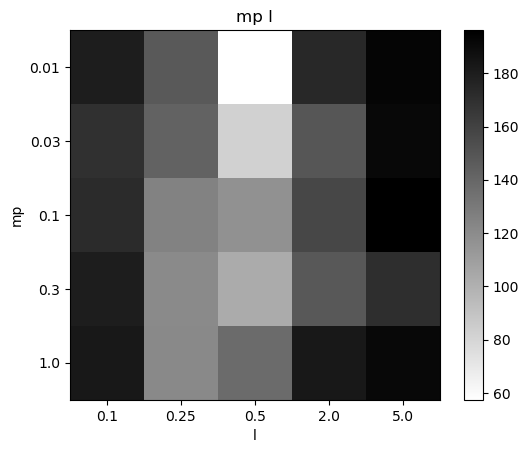
\includegraphics[width = 1.0\linewidth, trim={0 0 0 0}, clip=true]{figures/test_mp_l_heat.png}
		\subcaption{Performance for different pole masses (mp) and lengths (l).}
		\label{fig:mp_l}	
	\end{subfigure}
\caption{Learning performance as a function of different sets of parameters. The value given is the number of trials needed for the mean trial length to exceed 10,000 seconds of simulated time. Lower values indicate better performance. The simulations were capped at an upper limit of 200 trials.}
\label{fig:params}
\end{figure}

We see from figure \ref{fig:delta_lambda} that performance strongly depends on the eligibility trace decay rates $\delta$ and $\lambda$ with optimum performance observed for $\delta = 0.9$ and $\lambda = 0.6-0.8$. This is very similar to the parameters used by Barto et al. Performance drops at very low decay rates as it prevents the system from correctly penalizing recent states that lead to failure and performance drops at high decay rates as early states are penalized even if they are far removed from the failure of the system, leading to less differentiation between 'good' and 'bad' states.

On the contrary, the learning rates $\alpha$ and $\beta$ has surprisingly little effect on the performance of the system with a wide range of parameter values giving performances in the range 80-140 (figure \ref{fig:alpha_beta}). At very low $\alpha$ or $\beta$, the system fails to learn over the course of the simulation and performance deteriorates. At high $\beta$, the memory of the ACE deteriorates and performance gets worse. However, at very high $\alpha$ the behavior of the system saturates as we effectively get 'one-shot learning' in the ASE without a dorp in performance.

In figure \ref{fig:mp_l} we see that the performance is highly dependent on pole length (l) but less so on pole mass (mp). The task becomes easier as the pole becomes lighter since this leads to slower dynamics and thus less frequent pole drops. The task becomes harder when the pole becomes too short since $|\dot \theta|$ increases with decreasing $l$ ($\ddot \theta \propto 1/l$). It also becomes harder as the pole gets too long since $|\dot x|$ increases with increasing $l$. $l = 0.5$ represents a balance between these two effects. 

Having investigated the performance of this simple model, we can now add a second layer to the network  as inspired by Anderson (1987). We denote the activities of this hidden layer $z$ with weights from the input signal given by the matrix $D$. In this case, the input \textbf{x} is the full state vector scaled as described in Anderson et al. and with an additional bias unit with a constant value of 0.5.
\begin{equation}
z_i(t) = g(\sum_{j=1}{D_{ij}(t) x_j(t)})
\end{equation}
Where $g(s) = \dfrac{1}{1+e^{-s}}$. This allows us to calculate a probability
\begin{equation}
P(t) = g(\sum_{i=1}{w_{i}(t) x_i(t)} + \sum_{i=1}{f_i(t)z_i(t)})
\end{equation}
where $f_i$ are the weights from the hidden layer to the output layer (equivalent to $w_i$ for the input layer).
We then have $y(t) = 1$ with probability $P(t)$ and $y(t) = -1$ with probability $1-P(t)$.
Our ACE is also expanded by a hidden layer  $q$ with connectivity matrix $A$ from the input layer and activities
\begin{equation}
q_i(t1, t2) = g(\sum_{j=1}{A_{ij}(t1) x_j(t2)})
\end{equation}
\begin{equation}
p(t1,t2) = \sum_{i=1}{v_{i}(t1) x_i(t2)} + \sum_{i=1}{c_i(t1)q_i(t2)}
\end{equation}
This gives us an expected reward $\hat r = 0$ if the system is in a start state, $\hat r = r - p(t,t)$ if the system is in a failure state and $\hat r = r + \gamma p(t,t+1) - p(t,t)$ otherwise.
We then update the system weights according to
\begin{equation}
w_i(t+1) = w_i(t) + \alpha \hat r (t)(\max{(y(t), 0)} - P(t))x_i(t)
\end{equation}
\begin{equation}
f_i(t+1) = f_i(t) + \alpha \hat r (t)(\max{(y(t), 0)} - P(t))z_i(t)
\end{equation}
\begin{equation}
D_{ij}(t+1) = D_{ij}(t) + \alpha \hat r (t) z_i(t) (1-z_i(t))\text{sign}(f_i(t)) (\max{(y(t), 0)} - P(t))x_j(t)
\end{equation}
\begin{equation}
v_i(t+1) = v_i(t) + \beta \hat r (t) x_i(t)
\end{equation}
\begin{equation}
c_i(t+1) = c_i(t) + \beta \hat r (t) q_i(t,t)
\end{equation}
\begin{equation}
A_{ij}(t+1) = A_{ij}(t) + \beta \hat r (t) q_i(t,t) (1-q_i(t,t))\text{sign}(c_i(t)) x_j(t)
\end{equation}

in the present case, the additional layer does not significantly improve performance; however, Anderson had made the task more difficult by scaling, shifting and random initialization of the task and found that the second layer only improved performance after a large number of iterations. However, in the present simpler case, the network rapidly learns the task and the second layer is therefore not necessary.
%
%\begin{figure}[h]
%	\centering
%	\begin{subfigure}[t]{0.28\linewidth}
%		\centering
%		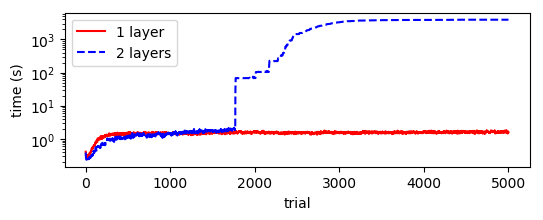
\includegraphics[width = 1.0\linewidth, trim={0 0 0 0}, clip=true]{figures/compare_layers.png}	
%	\end{subfigure}%
%\caption{Performance for 1 and 2 layers}
%\label{fig:cart_layers}
%\end{figure}

\newpage

\section*{Appendix}

%\lstinputlisting[language=python]{ce_a1.py}


\end{document}


